\documentclass[../main]{subfiles}
\newcommand*\circled[1]{\tikz[baseline=(char.base)]{
            \node[shape=circle,draw,inner sep=1pt] (char) {#1};}}
    \begin{document}
    \setcounter{secnumdepth}{2}
    \chapter{提案手法}
        \section{提案手法の概要}
        本研究は,全天球カメラから取得した画像に基づき,通路認識を行う手法の検証を行う.
        ここでいう通路認識とは,画像中に通路があるかどうかを認識するだけでなく,
        画像中に通路がある場合,その通路がどのタイプに属するのかといった,
        通路の特徴を抽出することである.
        また,本研究で扱う通路のタイプは以下の8種類である.それぞれの図を\fref{figure::new_aisle_type}に示す.\\\\
         \circled{1}一本道(straight)\\
         \circled{2}行き止まり(dead end)\\
         \circled{3}右のみ曲がれる角(right)\\
         \circled{4}左のみ曲がれる角(left)\\
         \circled{5}十字路(cross)\\
         \circled{6}右に曲がれる三叉路(3-way junction\_right)\\
         \circled{7}左に曲がれる三叉路(3-way junction\_left)\\
         \circled{8}突き当たりの三叉路(3-way junction\_center)
       
        \vskip\baselineskip
        \vskip\baselineskip

        本手法の通路認識の流れを\fref{figure::proposed_method_fig}に示す.
        まず,全天球カメラにより取得したRGBの画像配列データをYOLOの入力とし,
        出力されたバウンディングボックスとクラス確率の情報をもとに画像中に通路があるかどうかを検出する.
        画像中に通路が検出された場合,通路の座標位置に基づき,通路のタイプを決定する.

        %8タイプの通路の画像例
        \begin{figure}[H]
            \centering
            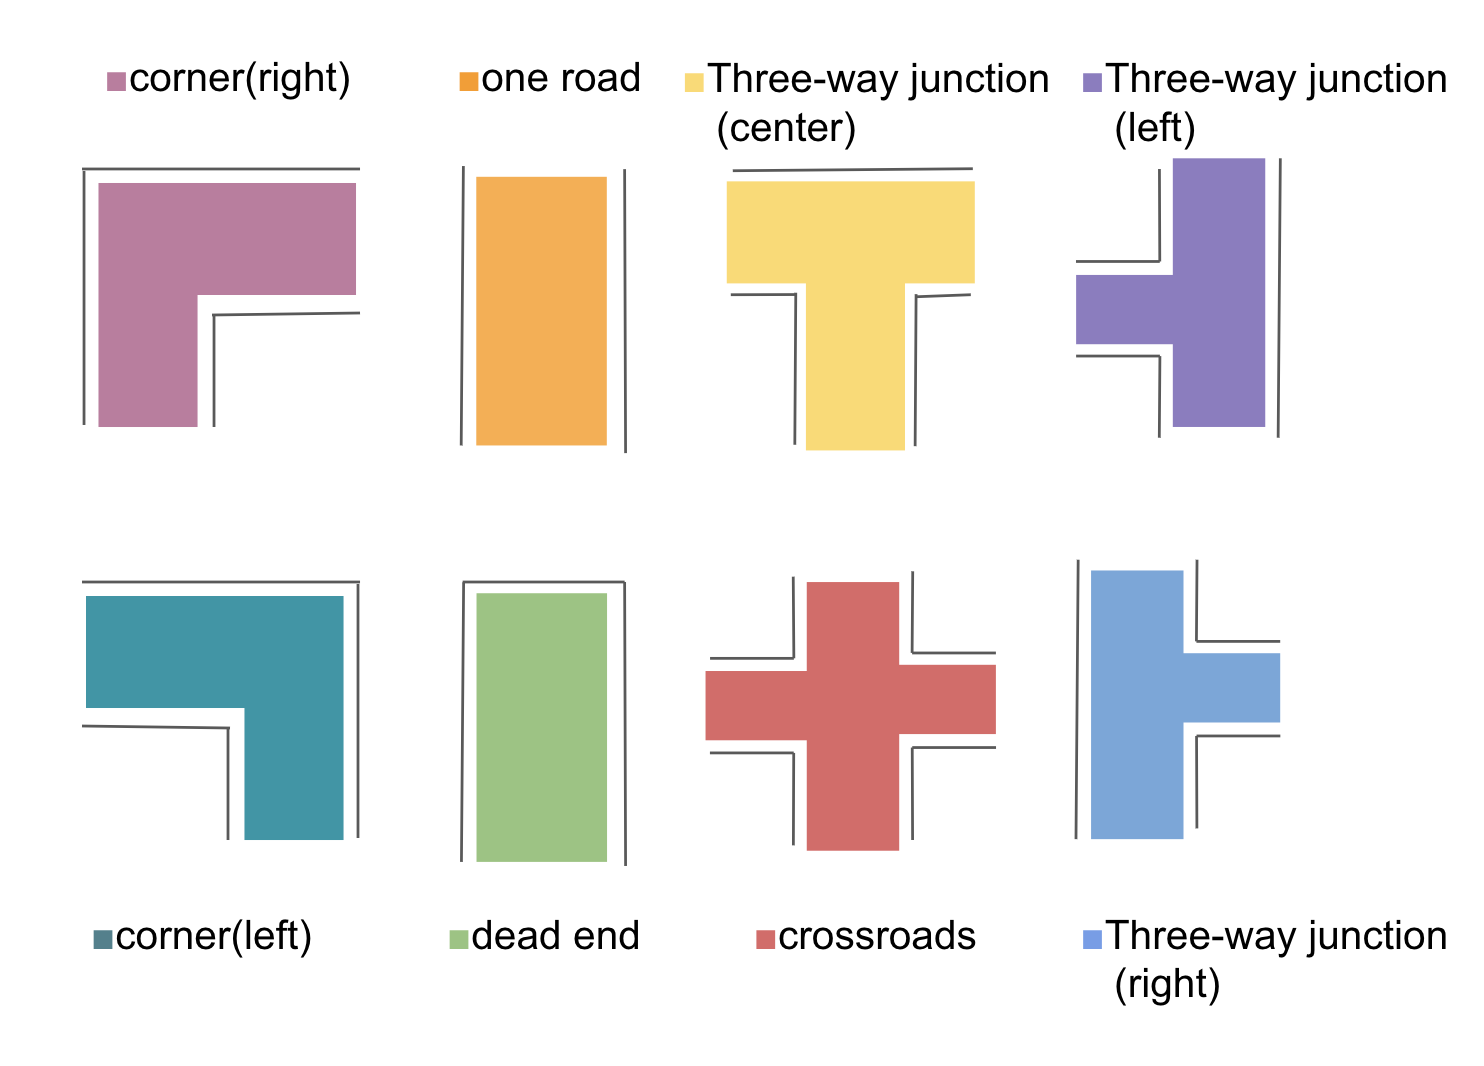
\includegraphics[width=10cm]{../images/new_aisle_type.png}
            \caption{Type of passage}
            \label{figure::new_aisle_type}
        \end{figure}
        
        %提案手法の簡単な例
        \begin{figure}[H]
            \centering
            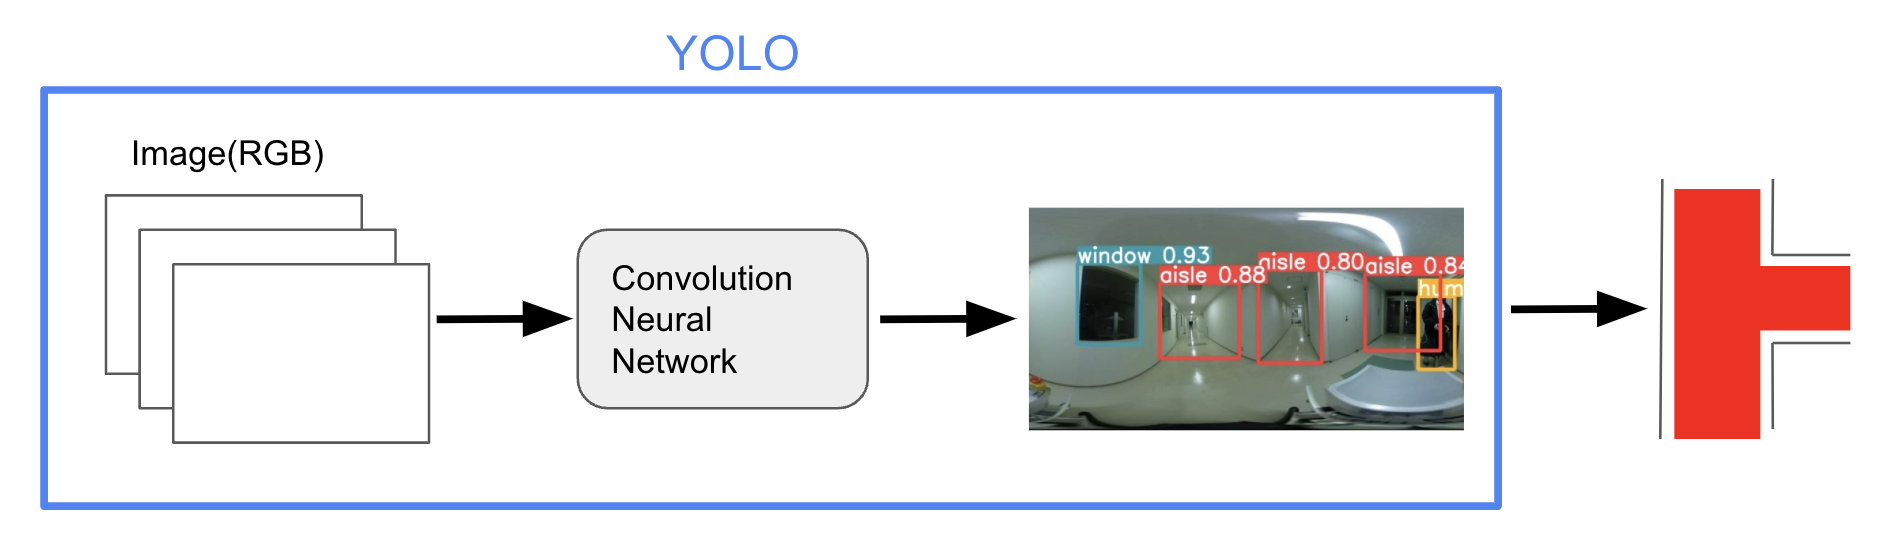
\includegraphics[width=15cm]{../images/proposed_method2.png}
            \caption{Flow of passage recognition method}
            \label{figure::proposed_method_fig}
            この例では,YOLOの出力した画像から通路が3つ検出されている.\\
            また,通路はロボットに対して前方,後方,右手側に検出されているため,\\
            通路のタイプは\circled{6}右に曲がれる三叉路であるということがわかる.
        \end{figure}

        \newpage

        \section{画像の前処理}
        全天球カメラで取得した画像は通常,\fref{subfigure::no_proc}に示すようにカメラの正面が画像の中心となり,後方の物体は画像の左端と右端で見切れてしまう.
        本手法では前後左右の通路を扱うため,見切れている状態は通路の認識精度に影響を与える恐れがある.そこで,YOLOに入力する前の段階で\fref{subfigure::preproc}
        に示すような画像の前処理を行う.
        画像の前処理としては以下のことを行う.
        ・画像のピクセル数を減らすため,960×1920から320×640の大きさにリサイズする
        ・カメラの前後左右全ての通路が画像内に収まるように,画像の左端1/8を切り取り右端にスライドさせる
    
        %画像の前処理の例
        \begin{figure}[htbp]
          \centering
           \subfigure[no processing image]{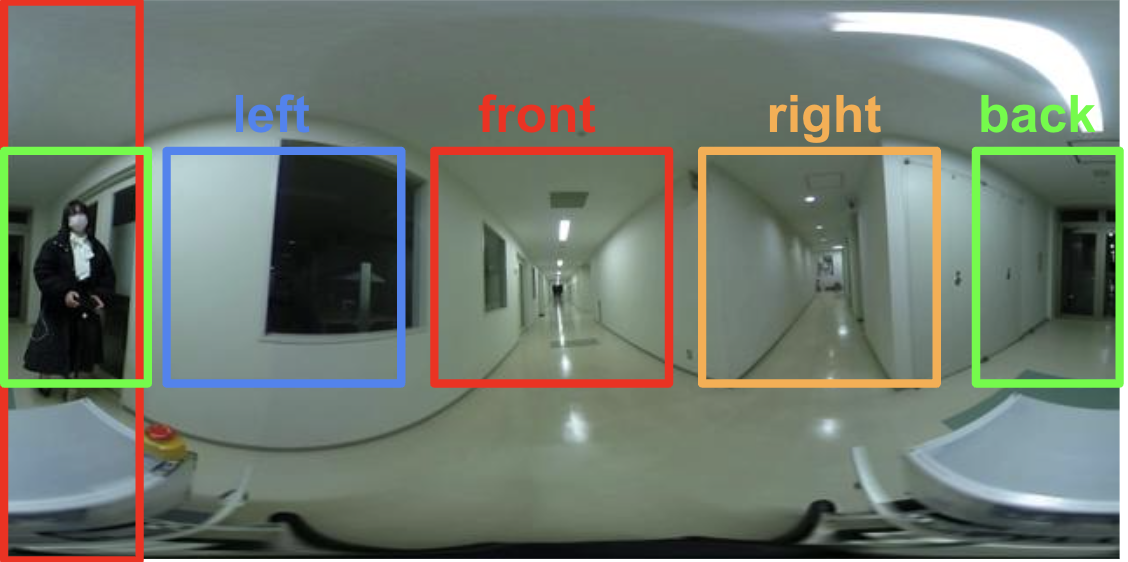
\includegraphics[height=4cm]{../images/no_processing.png}
           \label{subfigure::no_proc}}
           \subfigure[preprocessing image]{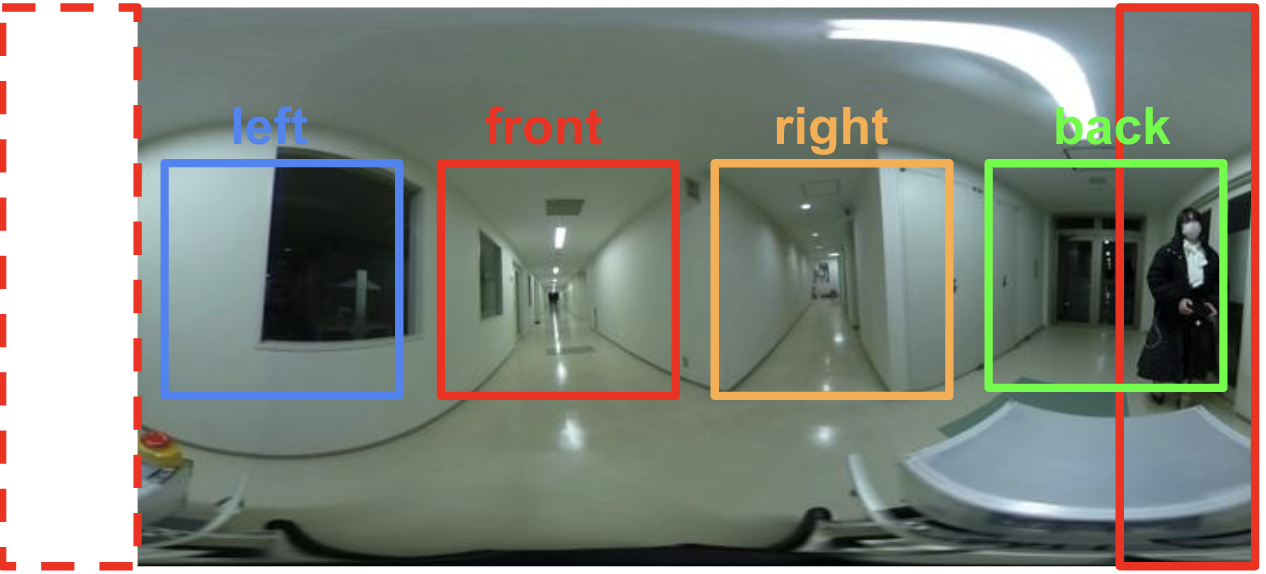
\includegraphics[height=4cm]{../images/after_processing.png}
           \label{subfigure::preproc}}
           \caption{Preprocessing of spherical camera images}
           \label{figure::proc_exp}
        \end{figure}
        
        \newpage

        \section{学習用データの作成}
        学習モデル作成のため,自作のデータセットにより学習を行う.学習に用いるデータは津田沼キャンパス2号館3階により収集し,作成した
        データセットの一部を\fref{figure::dataset_fig}に示す.データセットのラベル数は11クラスで設定し,クラス名を\tref{table::datasets_table}に示す.    

        %自作データセットの画像例
        \begin{figure}[H]
         \centering
         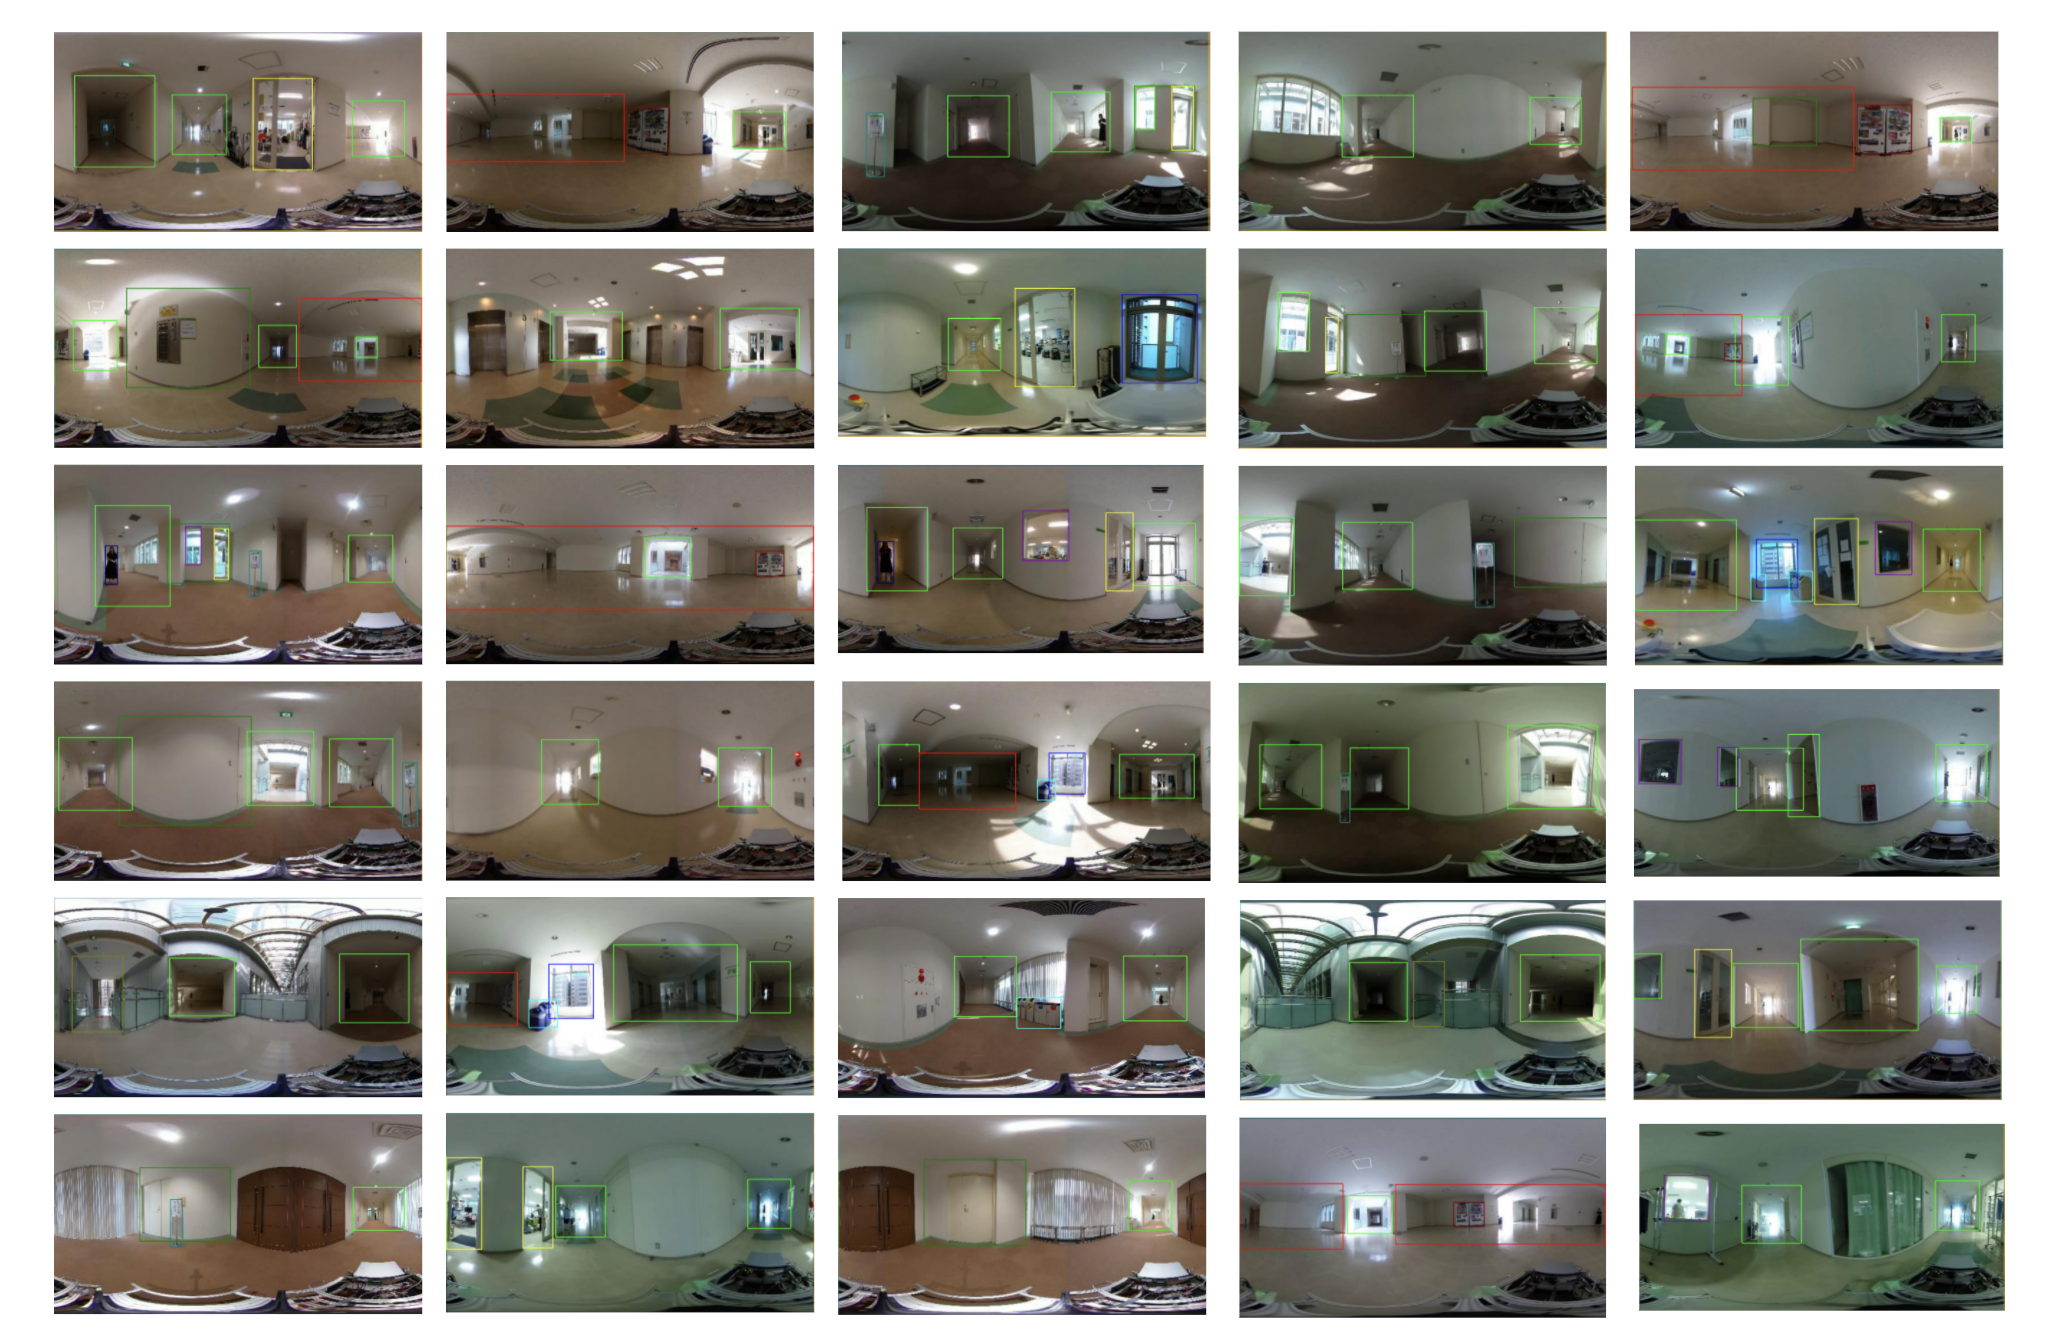
\includegraphics[width=10cm]{../images/dataset_exp.png}
         \caption{An example of a dataset.}
         \label{figure::dataset_fig}
        \end{figure}

        %データセットのクラス数
        \begin{table}[H]
            \caption{Class name to be labeled}
            \centering
            \label{table::datasets_table}
            \begin{tabular}{lllll}
            \hline
            name of the class &  &  &  &  \\ 
            \hline \hline
            aisle             &  &  &  &  \\
            end               &  &  &  &  \\
            door\_end         &  &  &  &  \\
            human             &  &  &  &  \\
            door              &  &  &  &  \\
            step              &  &  &  &  \\
            square            &  &  &  &  \\
            vending\_machine  &  &  &  &  \\
            trash\_can        &  &  &  &  \\
            signboard         &  &  &  &  \\
            window            &  &  &  &  \\ 
            \hline
            \end{tabular}
        \end{table}            

        \section{学習の結果}
        作成したデータセットを用いてYOLOv5により学習を行う.トレーニングに用いたネットワークを\fref{figure::}に示す.
        また,学習に用いるデータセットの構成を\fref{table::learning}に示す.

        \begin{table}[H]
            \caption{}
            \centering
            \label{table::learning}
            \begin{tabular}{l|l}
            \hline
            \multicolumn{1}{c|}{training}   & \multicolumn{1}{c|}{3540}                \\ \hline
            \multicolumn{1}{c|}{test}       & \multicolumn{1}{c|}{126}                  \\ \hline
            \multicolumn{1}{c|}{validation} & \multicolumn{1}{c|}{14}                  \\ \hline
            \multicolumn{1}{c|}{epoch}      & \multicolumn{1}{c|}{300}                \\ \hline
            \multicolumn{1}{c|}{batch}      & \multicolumn{1}{c|}{8}                   \\ \hline
            \end{tabular}
        \end{table}

\end{document}

%\begin{figure}[H]
        %\centering  
        %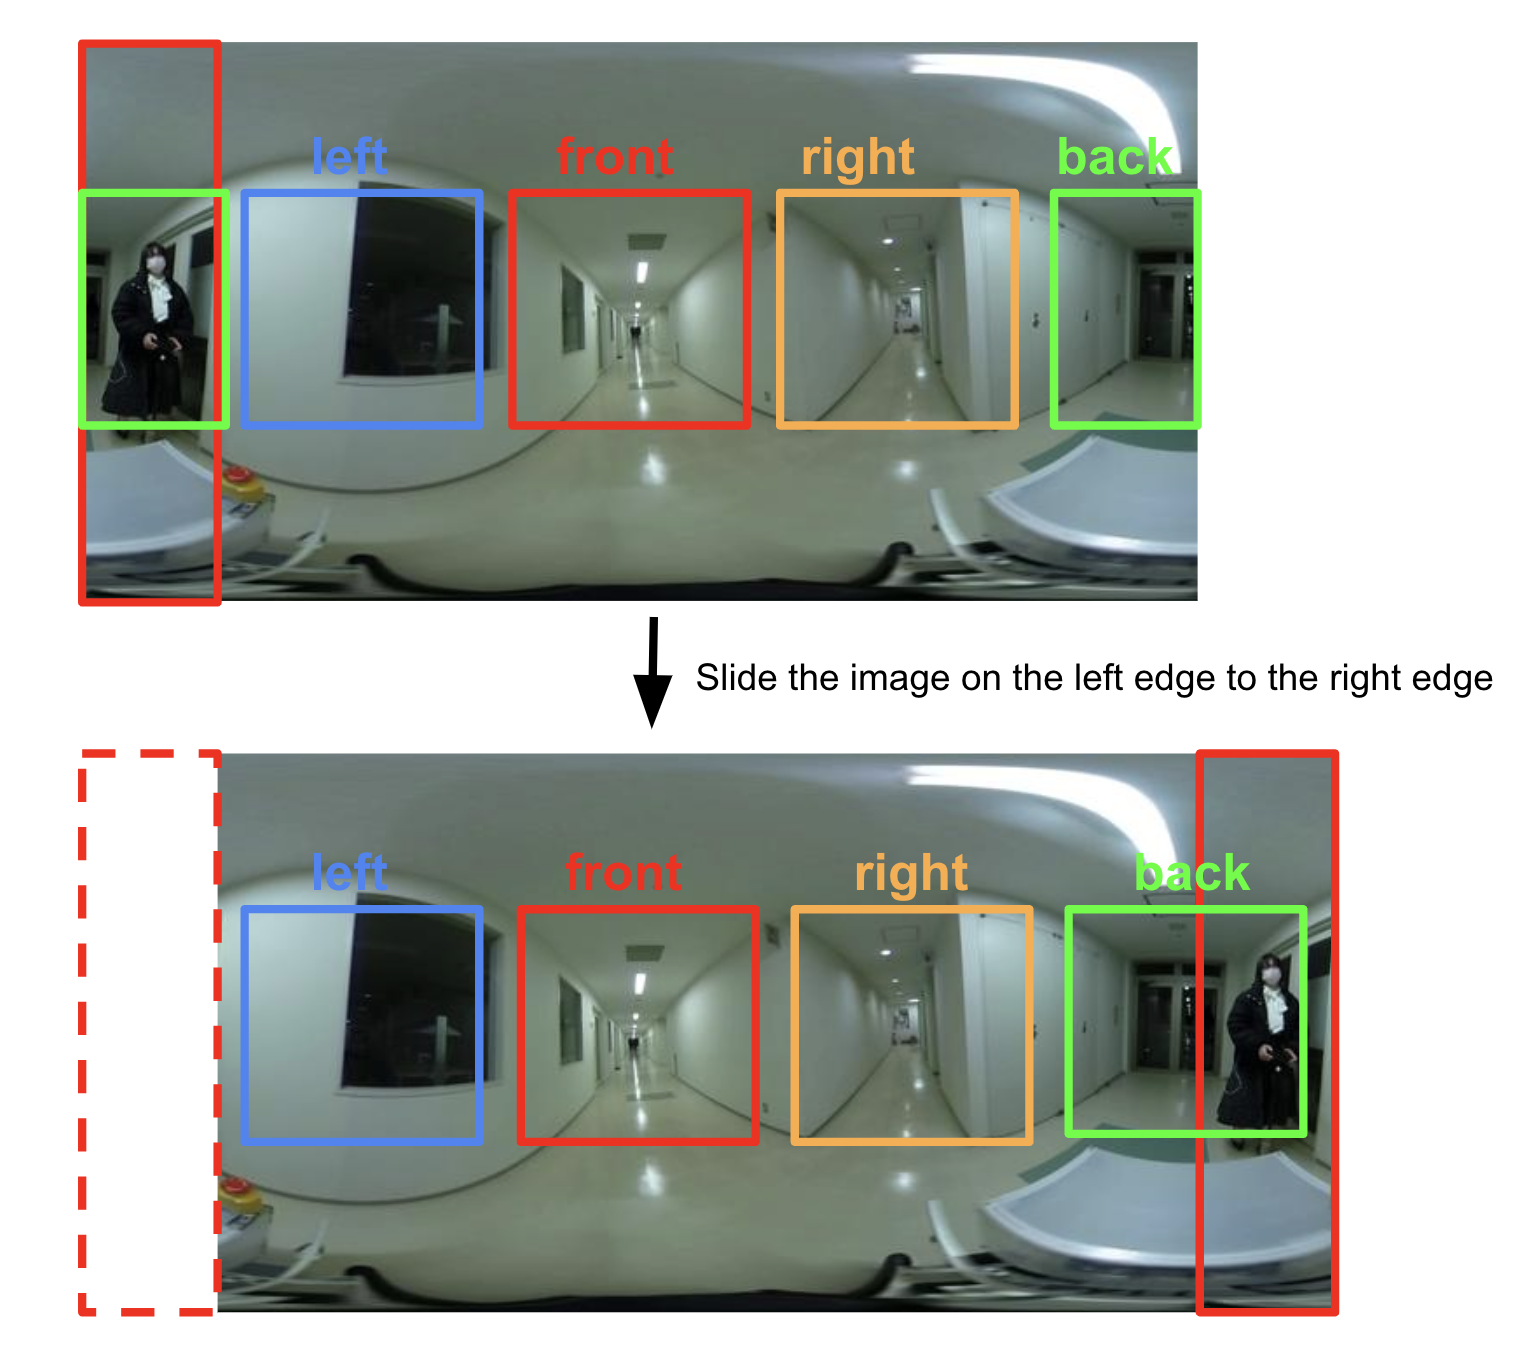
\includegraphics[width=10cm]{../images/image_proc2.png}
        %\caption{Preprocessing of spherical camera images.}
        %\label{figure::image_proc_fig}
        %\end{figure}